\documentclass{article}

% if you need to pass options to natbib, use, e.g.:
%     \PassOptionsToPackage{numbers, compress}{natbib}
% before loading neurips_2019

% ready for submission
% \usepackage{neurips_2019}

% to compile a preprint version, e.g., for submission to arXiv, add add the
% [preprint] option:
%     \usepackage[preprint]{neurips_2019}

% to compile a camera-ready version, add the [final] option, e.g.:
     \usepackage[final]{mlcb_2019}

% to avoid loading the natbib package, add option nonatbib:
%     \usepackage[nonatbib]{neurips_2019}

\usepackage[utf8]{inputenc} % allow utf-8 input
\usepackage[T1]{fontenc}    % use 8-bit T1 fonts
\usepackage{hyperref}       % hyperlinks
\usepackage{url}            % simple URL typesetting
\usepackage{booktabs}       % professional-quality tables
\usepackage{amsfonts}       % blackboard math symbols
\usepackage{nicefrac}       % compact symbols for 1/2, etc.
\usepackage{microtype}
\usepackage{amsmath}      % microtypography
\usepackage{bm}
\usepackage{graphicx}
\usepackage{verbatim}

\title{RNA Secondary Structure Prediction using Deep Neural Network}

% The \author macro works with any number of authors. There are two commands
% used to separate the names and addresses of multiple authors: \And and \AND.
%
% Using \And between authors leaves it to LaTeX to determine where to break the
% lines. Using \AND forces a line break at that point. So, if LaTeX puts 3 of 4
% authors names on the first line, and the last on the second line, try using
% \AND instead of \And before the third author name.

\author{%
  TODO \\
  Department of Electrical and Computer Engineering\\
  University of Toronto\\
  \texttt{todo@toronto.edu} \\
  % examples of more authors
  % \And
  % Coauthor \\
  % Affiliation \\
  % Address \\
  % \texttt{email} \\
  % \AND
  % Coauthor \\
  % Affiliation \\
  % Address \\
  % \texttt{email} \\
  % \And
  % Coauthor \\
  % Affiliation \\
  % Address \\
  % \texttt{email} \\
  % \And
  % Coauthor \\
  % Affiliation \\
  % Address \\
  % \texttt{email} \\
}

\begin{document}

\maketitle

\begin{abstract}
  TODO
\end{abstract}


\section{Introduction}

\begin{itemize}

    \item State-of-the-art methods based on dynamic programming.
Basic building blocks are known local structure, with their associated free energy measured experimentally.
Fixed energy parameters and hand-crafted rules.

    \item Emerging new dataset calls for flexible, extensible,
    end-to-end model that can be trained on new types of dataset (noisy, missing value).

    \item TODO review other papers using NN and discuss what's lacking.

\end{itemize}

%notation: we use ??? to represent a binary upper triangular matrix of size LxL.

\section{Method}

\subsection{Problem Formulation}

RNA secondary structure can be represented by a binary upper triangular matrix (excluding the diagonal).

As an example, a short RNA sequence GUUGUGAAAU of length $10$ (ID \verb|CRW_00083| TODO ref to database) takes a structure that
consists of a stem and a loop, as seen in Fig \ref{fig:rna_ss_binary_mat}(a).
This structure can be represented by the upper diagonal $10 \times 10$ matrix with all $0$'s,
except for positions $y_{1, 10}, y_{2, 9}$ and $y_{3, 8}$, all having value $1$.
This contiguous stretch of $1$'s corresponds to the stem formed by the three base pairs: G-U, U-A and U-A.
(TODO define x and y first)
(TODO cite FORNA)

\begin{figure}[h!]
    \centering
    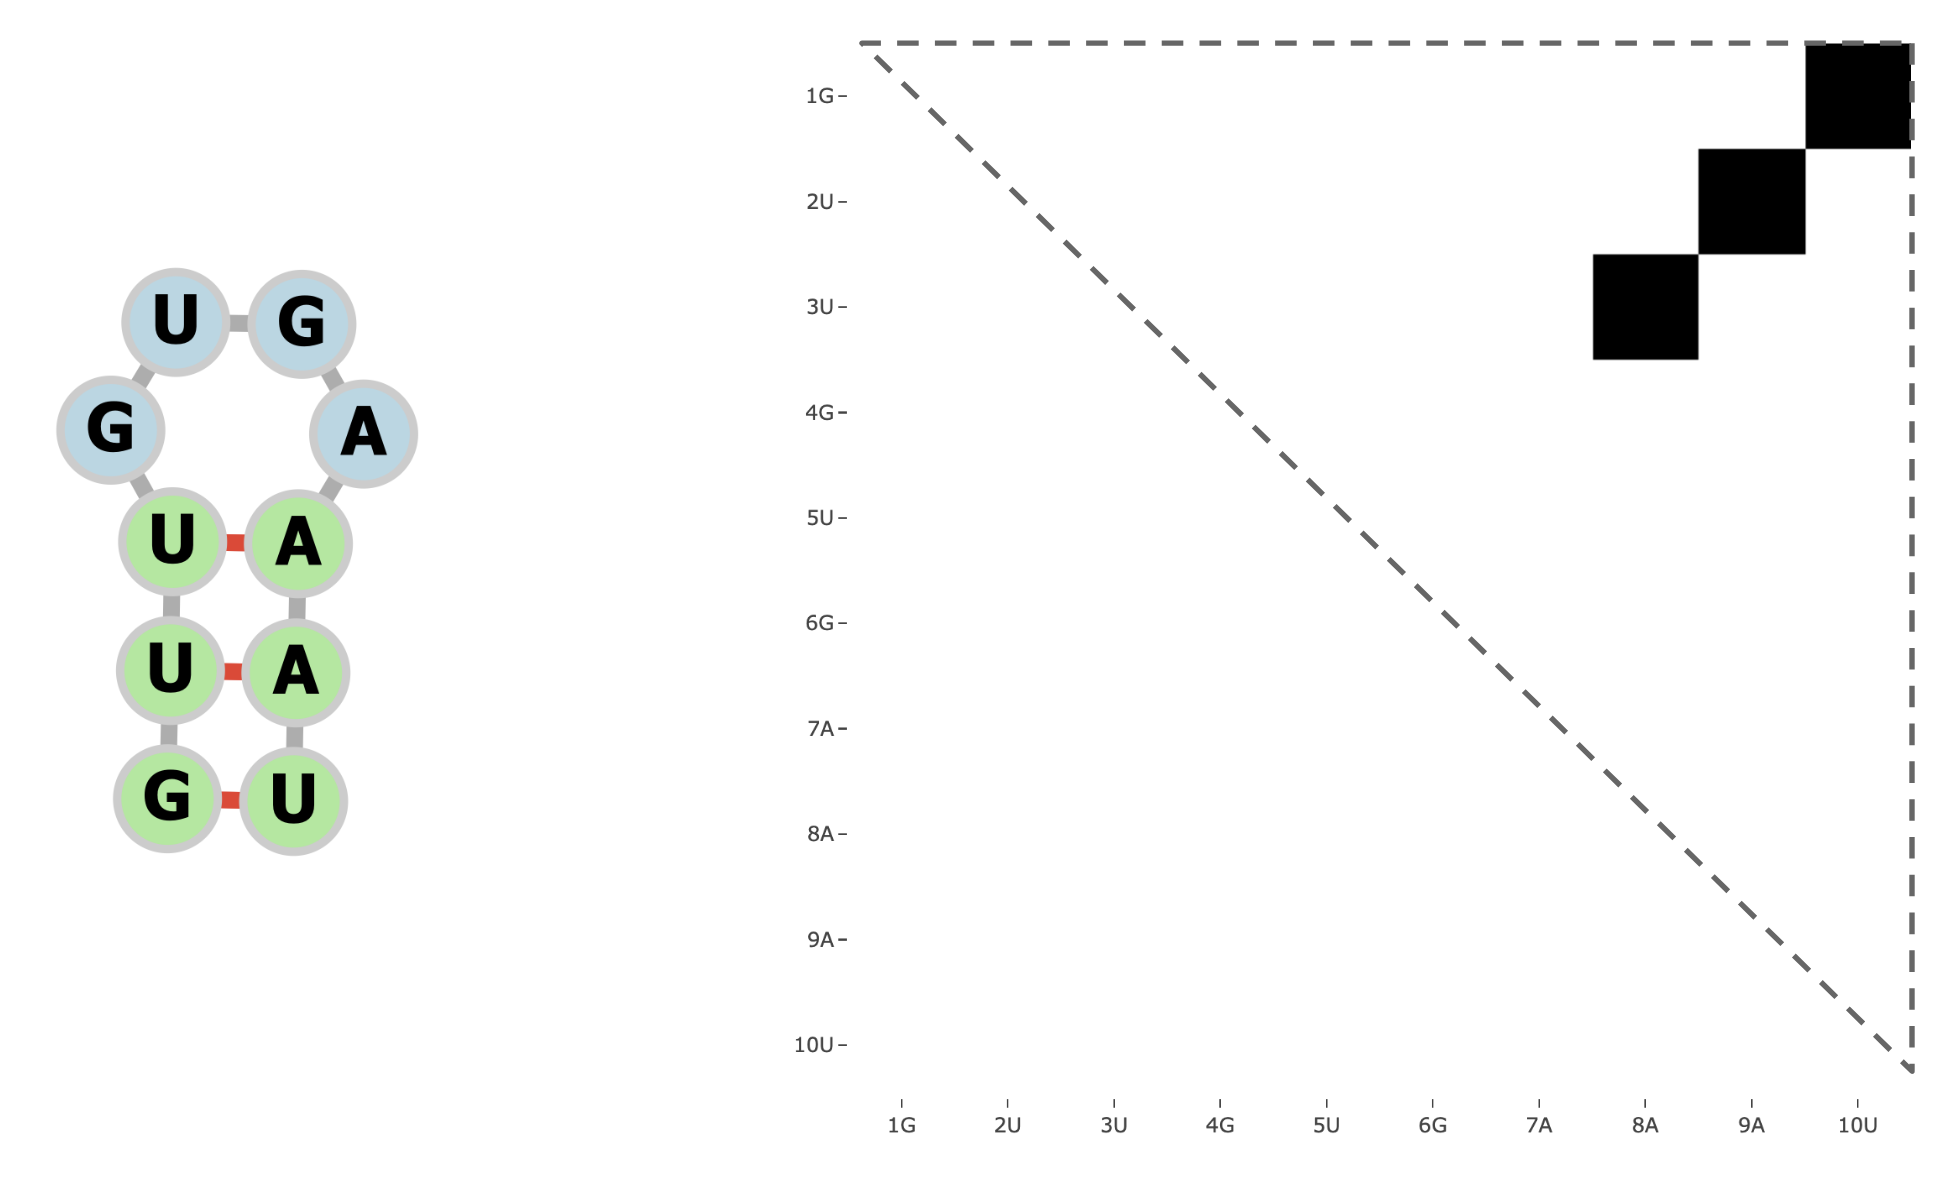
\includegraphics[width=0.5\textwidth]{plot/rna_ss_binary_mat.png}
    \caption{TODO}
    \label{fig:rna_ss_binary_mat}
    \centering
\end{figure}

We formulate the predictive task as a conditional generative process.
Specifically, given an input sequence with arbitrary length $L$: $\bm{x} = x_1, x_2, \dots x_{L}$,
we want to predict a distribution of structures conditioned on the sequence $P(\bm{Y} \mid \bm{x})$.

%(TODO use the above notation).

We factorize the conditional distribution as follows:

$$
P(\bm{Y} \mid \bm{x}) = P(\{y_{i, i+1}\}_{i=1, 2, \dots L-1} \mid \bm{x})
P(\{y_{i, i+2}\}_{i=1, 2, \dots L-2} \mid \bm{x}, \{y_{i, i+1}\}_{i=1, 2, \dots L-1})
\dots
P(y_{i, j} \mid \bm{x}, \{y_{todo}\})
$$

The generative process implied by such formulation is illustrated in Fig \ref{fig:autoregressive_direction}.
We generated one off diagonal slice at a time, conditioned on the input sequence,
starting from the one adjacent to the diagonal line, as shown in yellow on the plot.
When generating the second slice (in green), we condition on the input sequence and the generated values in the first slice (in yellow).
When generating the third one (in blue), we condition on the input sequence and both the yellow and green slices.
This process continues until we fill the upper triangular matrix,
where the last entry (in red TODO color plot) is generated conditioned on the input and the entire upper triangular matrix except for itself.

\begin{figure}[h!]
    \centering
    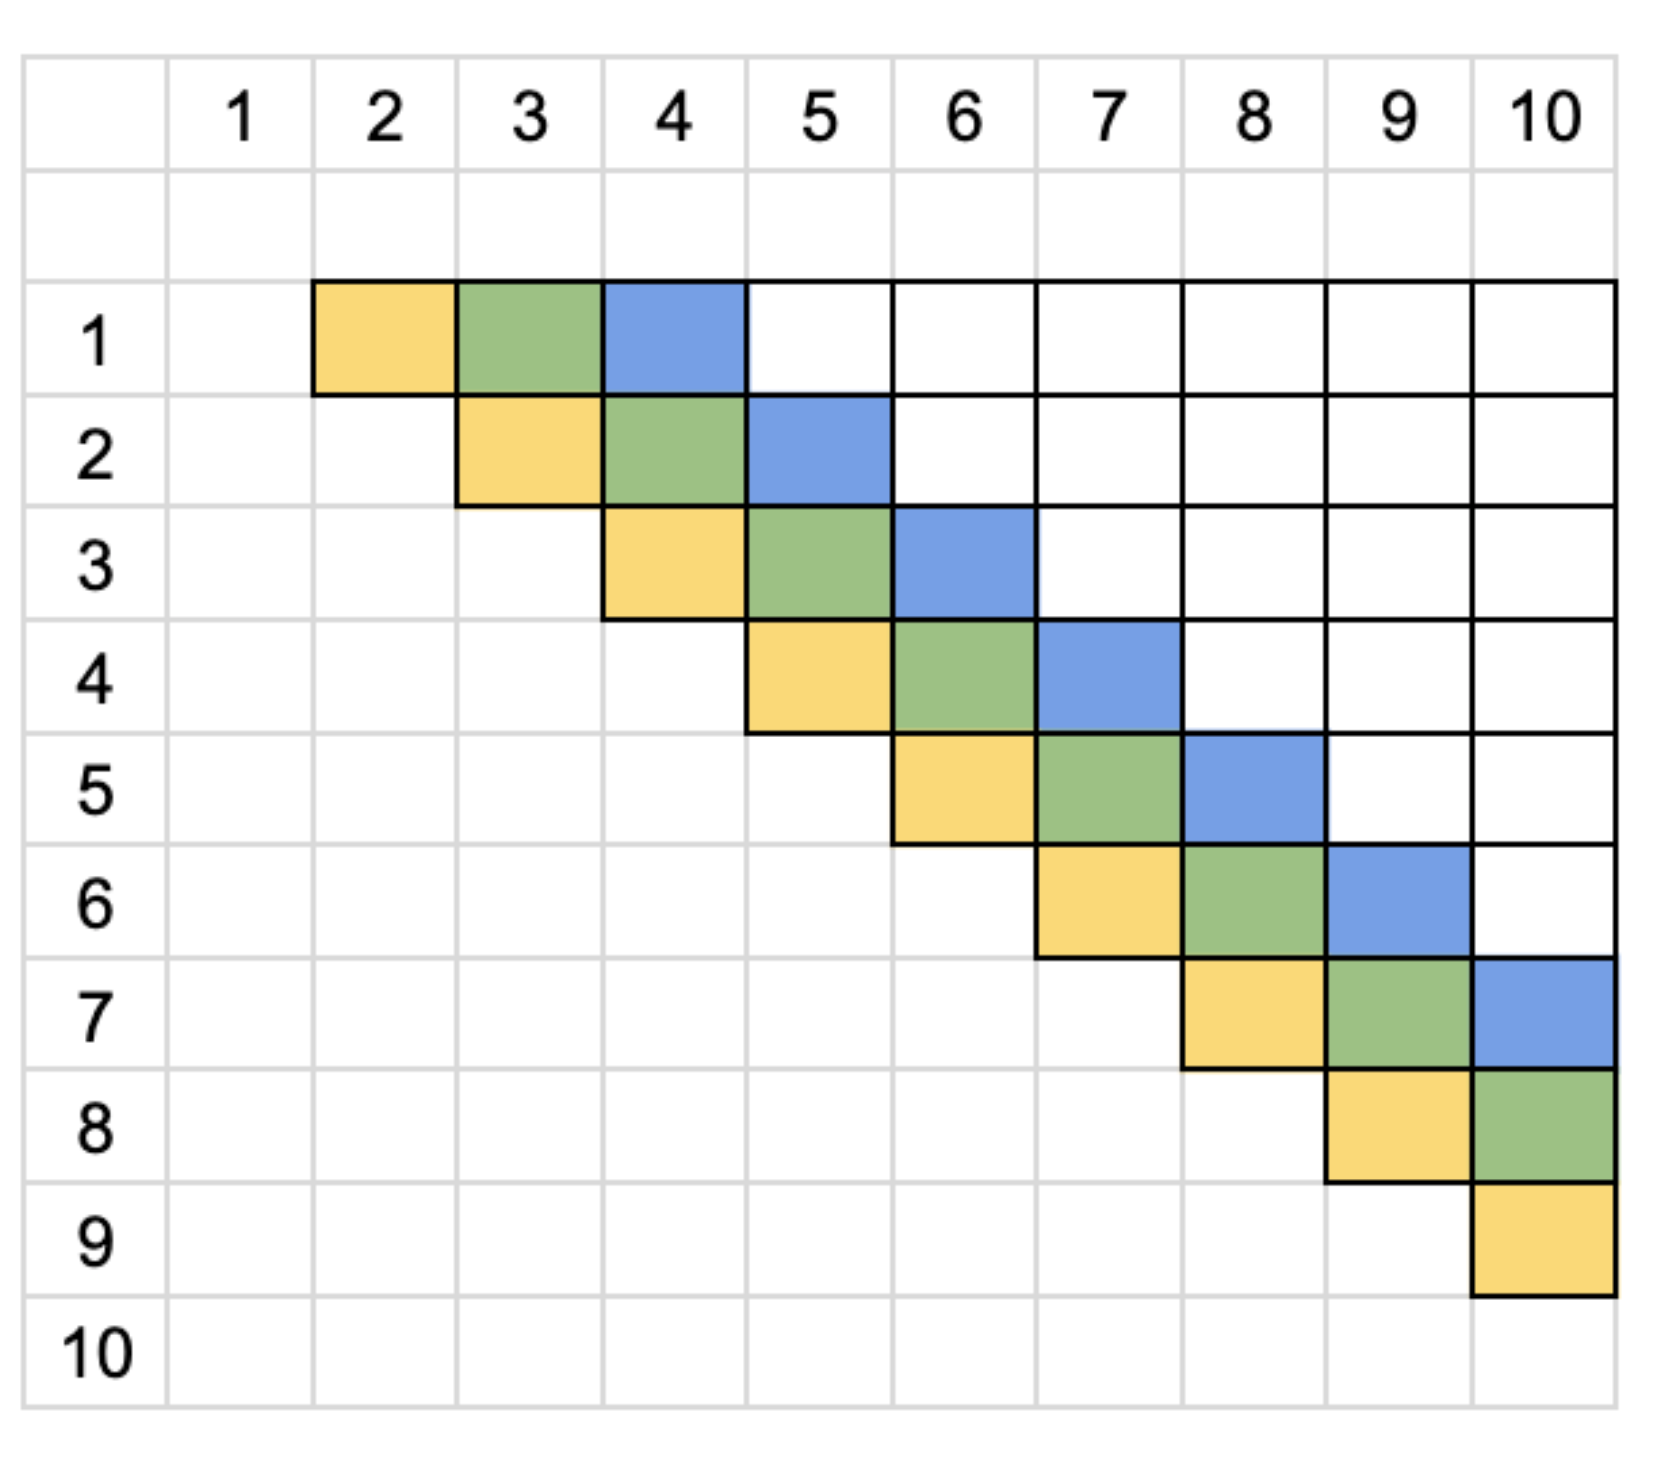
\includegraphics[width=0.5\textwidth]{plot/autoregressive_direction.png}
    \caption{TODO}
    \label{fig:autoregressive_direction}
    \centering
\end{figure}


%intuition, sample local connectivity then global?


\subsection{Model}

We propose an architecture that encourages learning
basic rules of base pairing and local structures, to construct the global structure,
without having hard-coded parameters,
such that the entire model can be learned end-to-end from sequence to structure.
The architecture consists of the following components:

%Incoporate biological knowledge.

\begin{itemize}

    \item two sets of 1D convolution layers on the 1-hot-encoded sequence

    \item Activations of each 1d conv layer (from both sets) are used to form a 2D feature map,
where the (i, j)-th entry is the dot-product (can be replaced by a fully connected NN) between the
activation of first set at position i, and the activation of second set at position j.

    \item Multiple 2D feature maps (formed via multiple layers of 1D conv) are concatenated,
followed by a couple of 2D conv layers.

    \item  Activation of the last 2D conv layer is concatenated with target from the previous "time-stamp" $y^{t-1}$ (todo define notation),
and the output is generated by an upper triangular convolution,
which masks "future" timestamps and ensure the output is generated in auto-regressive fashion. (TODO more details on masked conv)

    \item Finally, there is a fully connected layer along the feature (3rd) dimension,
   with sigmoid activation to produce an output between 0 and 1,
    for each position in the upper triangular matrix.

\end{itemize}

At training time, different timestamps can be trained in parallel.
At test time, we need to initialize the output at time $t=-1$, typically with a matrix of all zeros,
then sample one slice at a time, until the full upper triangular matrix is filled.
For a sequence of length $L-1$, we need to run $L-1$ steps sequentially.
Note that multiple outputs can be sampled in parallel at test time.


%To encourage learning of base-pairing and local structure formation,
%we construct 2D feature maps, each corresponds to a specific receptive window on 1D sequence.
%
%Entry (i, j) in each feature map is the output of


TODO plot for NN architecture

%batch, mask

\subsection{Training}

We trained the model using a synthetic dataset, constructed by sampling $50000$ random sequences with length
between $10$ and $100$.
For each sequence, we ran RNAfold (TODO ref) with the default parameters and
record the minimum free energy structure.

For each minibatch, we zero-pad the sequence array and structure matrix to the maximum length in the minibatch.
When computing the loss and gradient, entries in structure matrix that were padded are being masks,
in addition to the lower triangular entries (since we're only predicting the upper triangular matrix).

Note that although we present a single output structure for each input sequence at training time,
the model is capable of generating a distribution of structures at test time.

TODO hyperparameters

%Special constraints when sampling the matrix.

%Describe dataset.

%1-step AR.

\subsection{Sampling structures}

At test time, we can sample structures conditioned on the input sequence.
As described in Section ?, we initialize the output structure with a matrix of all zeros,
then sample one slice at a time until the upper triangular matrix is filled with sampled values.
At each step, we sample a binary label for each position in the current slice based on the
bernoulli probability predicted by the model.
To ensure the sampled structure is valid, when sampling the label for location (i, j),
if i-th or j-th position is already paired with another position (from samples in the previous timestamps),
then we set $y_{i, j}$ to $0$ without sampling from the model output.

\section{Analysis}

\subsection{Generate distribution of structures}

As an example, for a 323-base long sequence (TODO link to DB),
we sampled 20 structure from the model output, as shown in Fig \ref{fig:sampled_structures}.
On the left we show the binary upper triangular matrix sampled by the model (TODO it's too tiny to see anything),
on the right we show the corresponding secondary structure rendered as a graph (only showing 4 due to space limit).


\begin{figure}[h!]
    \centering
    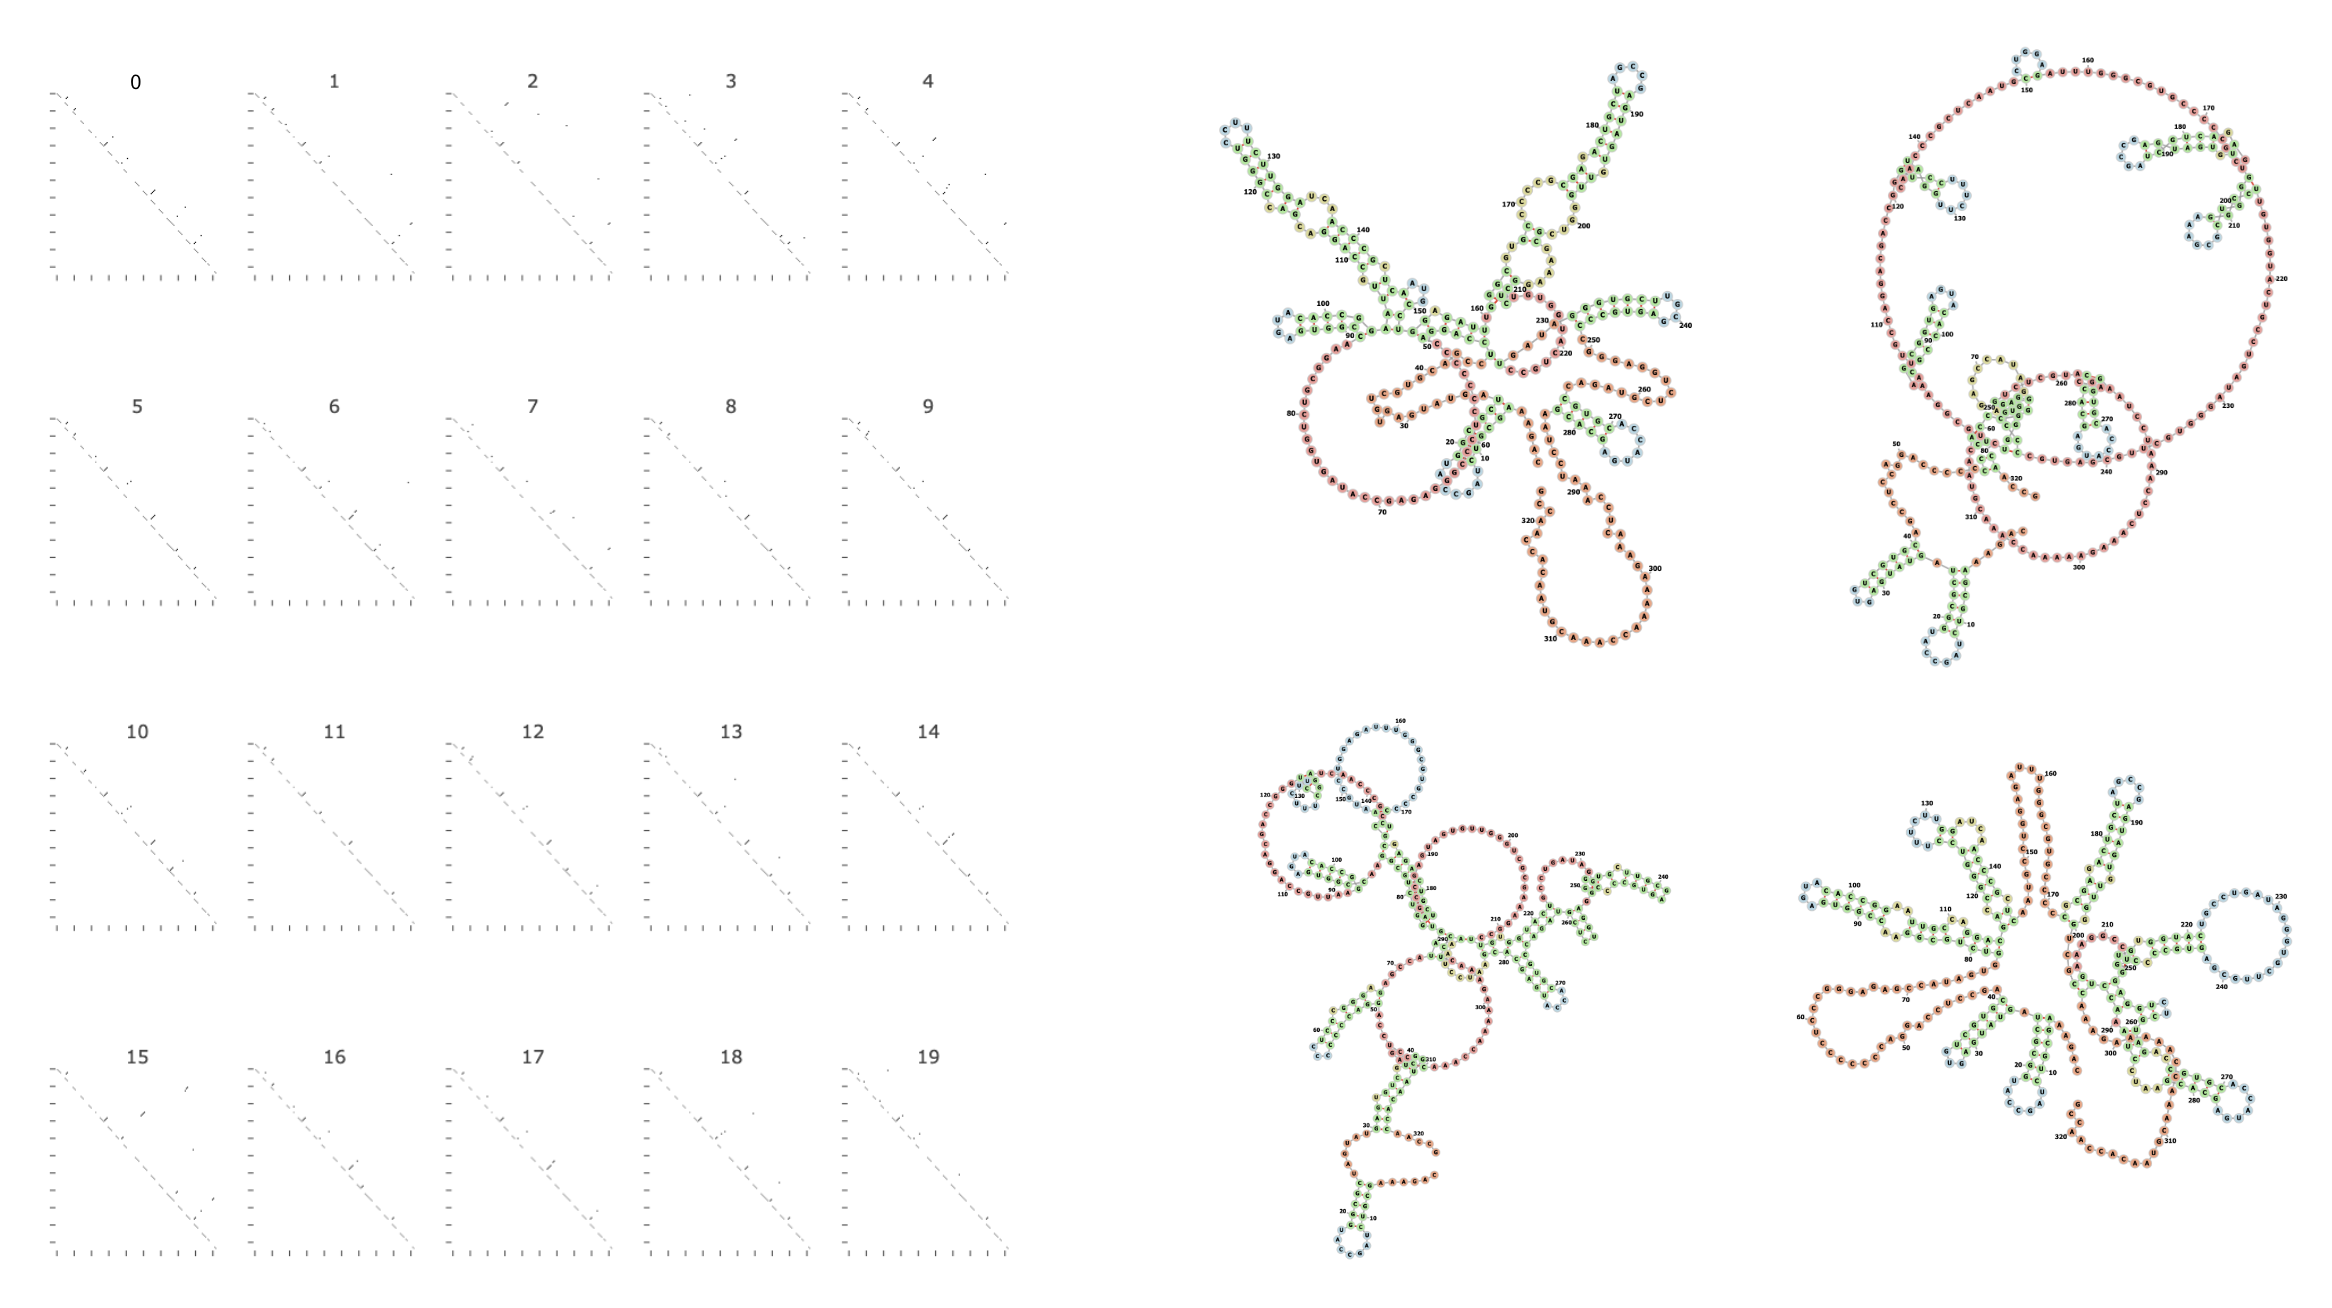
\includegraphics[width=\textwidth]{plot/sampled_structures.png}
    \caption{TODO}
    \label{fig:sampled_structures}
    \centering
\end{figure}



%TODO show generating an ensemble of structures

\subsection{Run time comparison}

\subsection{Performance comparison}

\subsection{Interesting cases}

\subsection{Differentiable model}

%differentialble model. use case.

\section{Conclusion}


%Speed consideration: implement split architecture, only need one forward pass for up to the last layer,
%then run last layer (triangular convolution) for $L-1$ times.
%
%
%Case study:
%
%TODO compare with RNAfold performance
%
%TODO reference on a new page


%\section{Submission of papers to NeurIPS 2019}
%
%NeurIPS requires electronic submissions.  The electronic submission site is
%\begin{center}
%  \url{https://cmt.research.microsoft.com/NeurIPS2019/}
%\end{center}
%
%Please read the instructions below carefully and follow them faithfully.
%
%\subsection{Style}
%
%Papers to be submitted to NeurIPS 2019 must be prepared according to the
%instructions presented here. Papers may only be up to eight pages long,
%including figures. Additional pages \emph{containing only acknowledgments and/or
%  cited references} are allowed. Papers that exceed eight pages of content
%(ignoring references) will not be reviewed, or in any other way considered for
%presentation at the conference.
%
%The margins in 2019 are the same as since 2007, which allow for $\sim$$15\%$
%more words in the paper compared to earlier years.
%
%Authors are required to use the NeurIPS \LaTeX{} style files obtainable at the
%NeurIPS website as indicated below. Please make sure you use the current files
%and not previous versions. Tweaking the style files may be grounds for
%rejection.
%
%\subsection{Retrieval of style files}
%
%The style files for NeurIPS and other conference information are available on
%the World Wide Web at
%\begin{center}
%  \url{http://www.neurips.cc/}
%\end{center}
%The file \verb+neurips_2019.pdf+ contains these instructions and illustrates the
%various formatting requirements your NeurIPS paper must satisfy.
%
%The only supported style file for NeurIPS 2019 is \verb+neurips_2019.sty+,
%rewritten for \LaTeXe{}.  \textbf{Previous style files for \LaTeX{} 2.09,
%  Microsoft Word, and RTF are no longer supported!}
%
%The \LaTeX{} style file contains three optional arguments: \verb+final+, which
%creates a camera-ready copy, \verb+preprint+, which creates a preprint for
%submission to, e.g., arXiv, and \verb+nonatbib+, which will not load the
%\verb+natbib+ package for you in case of package clash.
%
%\paragraph{Preprint option}
%If you wish to post a preprint of your work online, e.g., on arXiv, using the
%NeurIPS style, please use the \verb+preprint+ option. This will create a
%nonanonymized version of your work with the text ``Preprint. Work in progress.''
%in the footer. This version may be distributed as you see fit. Please \textbf{do
%  not} use the \verb+final+ option, which should \textbf{only} be used for
%papers accepted to NeurIPS.
%
%At submission time, please omit the \verb+final+ and \verb+preprint+
%options. This will anonymize your submission and add line numbers to aid
%review. Please do \emph{not} refer to these line numbers in your paper as they
%will be removed during generation of camera-ready copies.
%
%The file \verb+neurips_2019.tex+ may be used as a ``shell'' for writing your
%paper. All you have to do is replace the author, title, abstract, and text of
%the paper with your own.
%
%The formatting instructions contained in these style files are summarized in
%Sections \ref{gen_inst}, \ref{headings}, and \ref{others} below.
%
%\section{General formatting instructions}
%\label{gen_inst}
%
%The text must be confined within a rectangle 5.5~inches (33~picas) wide and
%9~inches (54~picas) long. The left margin is 1.5~inch (9~picas).  Use 10~point
%type with a vertical spacing (leading) of 11~points.  Times New Roman is the
%preferred typeface throughout, and will be selected for you by default.
%Paragraphs are separated by \nicefrac{1}{2}~line space (5.5 points), with no
%indentation.
%
%The paper title should be 17~point, initial caps/lower case, bold, centered
%between two horizontal rules. The top rule should be 4~points thick and the
%bottom rule should be 1~point thick. Allow \nicefrac{1}{4}~inch space above and
%below the title to rules. All pages should start at 1~inch (6~picas) from the
%top of the page.
%
%For the final version, authors' names are set in boldface, and each name is
%centered above the corresponding address. The lead author's name is to be listed
%first (left-most), and the co-authors' names (if different address) are set to
%follow. If there is only one co-author, list both author and co-author side by
%side.
%
%Please pay special attention to the instructions in Section \ref{others}
%regarding figures, tables, acknowledgments, and references.
%
%\section{Headings: first level}
%\label{headings}
%
%All headings should be lower case (except for first word and proper nouns),
%flush left, and bold.
%
%First-level headings should be in 12-point type.
%
%\subsection{Headings: second level}
%
%Second-level headings should be in 10-point type.
%
%\subsubsection{Headings: third level}
%
%Third-level headings should be in 10-point type.
%
%\paragraph{Paragraphs}
%
%There is also a \verb+\paragraph+ command available, which sets the heading in
%bold, flush left, and inline with the text, with the heading followed by 1\,em
%of space.
%
%\section{Citations, figures, tables, references}
%\label{others}
%
%These instructions apply to everyone.
%
%\subsection{Citations within the text}
%
%The \verb+natbib+ package will be loaded for you by default.  Citations may be
%author/year or numeric, as long as you maintain internal consistency.  As to the
%format of the references themselves, any style is acceptable as long as it is
%used consistently.
%
%The documentation for \verb+natbib+ may be found at
%\begin{center}
%  \url{http://mirrors.ctan.org/macros/latex/contrib/natbib/natnotes.pdf}
%\end{center}
%Of note is the command \verb+\citet+, which produces citations appropriate for
%use in inline text.  For example,
%\begin{verbatim}
%   \citet{hasselmo} investigated\dots
%\end{verbatim}
%produces
%\begin{quote}
%  Hasselmo, et al.\ (1995) investigated\dots
%\end{quote}
%
%If you wish to load the \verb+natbib+ package with options, you may add the
%following before loading the \verb+neurips_2019+ package:
%\begin{verbatim}
%   \PassOptionsToPackage{options}{natbib}
%\end{verbatim}
%
%If \verb+natbib+ clashes with another package you load, you can add the optional
%argument \verb+nonatbib+ when loading the style file:
%\begin{verbatim}
%   \usepackage[nonatbib]{neurips_2019}
%\end{verbatim}
%
%As submission is double blind, refer to your own published work in the third
%person. That is, use ``In the previous work of Jones et al.\ [4],'' not ``In our
%previous work [4].'' If you cite your other papers that are not widely available
%(e.g., a journal paper under review), use anonymous author names in the
%citation, e.g., an author of the form ``A.\ Anonymous.''
%
%\subsection{Footnotes}
%
%Footnotes should be used sparingly.  If you do require a footnote, indicate
%footnotes with a number\footnote{Sample of the first footnote.} in the
%text. Place the footnotes at the bottom of the page on which they appear.
%Precede the footnote with a horizontal rule of 2~inches (12~picas).
%
%Note that footnotes are properly typeset \emph{after} punctuation
%marks.\footnote{As in this example.}
%
%\subsection{Figures}
%
%\begin{figure}
%  \centering
%  \fbox{\rule[-.5cm]{0cm}{4cm} \rule[-.5cm]{4cm}{0cm}}
%  \caption{Sample figure caption.}
%\end{figure}
%
%All artwork must be neat, clean, and legible. Lines should be dark enough for
%purposes of reproduction. The figure number and caption always appear after the
%figure. Place one line space before the figure caption and one line space after
%the figure. The figure caption should be lower case (except for first word and
%proper nouns); figures are numbered consecutively.
%
%You may use color figures.  However, it is best for the figure captions and the
%paper body to be legible if the paper is printed in either black/white or in
%color.
%
%\subsection{Tables}
%
%All tables must be centered, neat, clean and legible.  The table number and
%title always appear before the table.  See Table~\ref{sample-table}.
%
%Place one line space before the table title, one line space after the
%table title, and one line space after the table. The table title must
%be lower case (except for first word and proper nouns); tables are
%numbered consecutively.
%
%Note that publication-quality tables \emph{do not contain vertical rules.} We
%strongly suggest the use of the \verb+booktabs+ package, which allows for
%typesetting high-quality, professional tables:
%\begin{center}
%  \url{https://www.ctan.org/pkg/booktabs}
%\end{center}
%This package was used to typeset Table~\ref{sample-table}.
%
%\begin{table}
%  \caption{Sample table title}
%  \label{sample-table}
%  \centering
%  \begin{tabular}{lll}
%    \toprule
%    \multicolumn{2}{c}{Part}                   \\
%    \cmidrule(r){1-2}
%    Name     & Description     & Size ($\mu$m) \\
%    \midrule
%    Dendrite & Input terminal  & $\sim$100     \\
%    Axon     & Output terminal & $\sim$10      \\
%    Soma     & Cell body       & up to $10^6$  \\
%    \bottomrule
%  \end{tabular}
%\end{table}
%
%\section{Final instructions}
%
%Do not change any aspects of the formatting parameters in the style files.  In
%particular, do not modify the width or length of the rectangle the text should
%fit into, and do not change font sizes (except perhaps in the
%\textbf{References} section; see below). Please note that pages should be
%numbered.
%
%\section{Preparing PDF files}
%
%Please prepare submission files with paper size ``US Letter,'' and not, for
%example, ``A4.''
%
%Fonts were the main cause of problems in the past years. Your PDF file must only
%contain Type 1 or Embedded TrueType fonts. Here are a few instructions to
%achieve this.
%
%\begin{itemize}
%
%\item You should directly generate PDF files using \verb+pdflatex+.
%
%\item You can check which fonts a PDF files uses.  In Acrobat Reader, select the
%  menu Files$>$Document Properties$>$Fonts and select Show All Fonts. You can
%  also use the program \verb+pdffonts+ which comes with \verb+xpdf+ and is
%  available out-of-the-box on most Linux machines.
%
%\item The IEEE has recommendations for generating PDF files whose fonts are also
%  acceptable for NeurIPS. Please see
%  \url{http://www.emfield.org/icuwb2010/downloads/IEEE-PDF-SpecV32.pdf}
%
%\item \verb+xfig+ "patterned" shapes are implemented with bitmap fonts.  Use
%  "solid" shapes instead.
%
%\item The \verb+\bbold+ package almost always uses bitmap fonts.  You should use
%  the equivalent AMS Fonts:
%\begin{verbatim}
%   \usepackage{amsfonts}
%\end{verbatim}
%followed by, e.g., \verb+\mathbb{R}+, \verb+\mathbb{N}+, or \verb+\mathbb{C}+
%for $\mathbb{R}$, $\mathbb{N}$ or $\mathbb{C}$.  You can also use the following
%workaround for reals, natural and complex:
%\begin{verbatim}
%   \newcommand{\RR}{I\!\!R} %real numbers
%   \newcommand{\Nat}{I\!\!N} %natural numbers
%   \newcommand{\CC}{I\!\!\!\!C} %complex numbers
%\end{verbatim}
%Note that \verb+amsfonts+ is automatically loaded by the \verb+amssymb+ package.
%
%\end{itemize}
%
%If your file contains type 3 fonts or non embedded TrueType fonts, we will ask
%you to fix it.
%
%\subsection{Margins in \LaTeX{}}
%
%Most of the margin problems come from figures positioned by hand using
%\verb+\special+ or other commands. We suggest using the command
%\verb+\includegraphics+ from the \verb+graphicx+ package. Always specify the
%figure width as a multiple of the line width as in the example below:
%\begin{verbatim}
%   \usepackage[pdftex]{graphicx} ...
%   \includegraphics[width=0.8\linewidth]{myfile.pdf}
%\end{verbatim}
%See Section 4.4 in the graphics bundle documentation
%(\url{http://mirrors.ctan.org/macros/latex/required/graphics/grfguide.pdf})
%
%A number of width problems arise when \LaTeX{} cannot properly hyphenate a
%line. Please give LaTeX hyphenation hints using the \verb+\-+ command when
%necessary.
%
%\subsubsection*{Acknowledgments}
%
%Use unnumbered third level headings for the acknowledgments. All acknowledgments
%go at the end of the paper. Do not include acknowledgments in the anonymized
%submission, only in the final paper.

%\section*{References}
%
%References follow the acknowledgments. Use unnumbered first-level heading for
%the references. Any choice of citation style is acceptable as long as you are
%consistent. It is permissible to reduce the font size to \verb+small+ (9 point)
%when listing the references. {\bf Remember that you can use more than eight
%  pages as long as the additional pages contain \emph{only} cited references.}
%\medskip
%
%\small
%
%[1] Alexander, J.A.\ \& Mozer, M.C.\ (1995) Template-based algorithms for
%connectionist rule extraction. In G.\ Tesauro, D.S.\ Touretzky and T.K.\ Leen
%(eds.), {\it Advances in Neural Information Processing Systems 7},
%pp.\ 609--616. Cambridge, MA: MIT Press.
%
%[2] Bower, J.M.\ \& Beeman, D.\ (1995) {\it The Book of GENESIS: Exploring
%  Realistic Neural Models with the GEneral NEural SImulation System.}  New York:
%TELOS/Springer--Verlag.
%
%[3] Hasselmo, M.E., Schnell, E.\ \& Barkai, E.\ (1995) Dynamics of learning and
%recall at excitatory recurrent synapses and cholinergic modulation in rat
%hippocampal region CA3. {\it Journal of Neuroscience} {\bf 15}(7):5249-5262.

\end{document}
